\chapter{Servidor de mapas dinámico}
\label{cap:sevidordemapasdinamico}


En este capítulo se explica la construcción y el funcionamiento del servidor de mapas dinámico. En primer lugar se explica que és, para que se utiliza y como se construye un \textit{costmap}. En segundo lugar se explica como se construyen los mapas que componen el algoritmo y por último se explica como se combinan estos mapas para generar el mapa usado en la navegación.

\section{Costmap\_2D}
\label{sec:costmap2d}
Un \textit{costmap} es una estructura de datos ofrecida por ROS y compuesta por un grid de ocupación y los metadatos de este grid. Cada celda del grid toma valores entre 0 y 255, donde 0 corresponde a una celda vacía, los valores entre 1 y 254 representan la probabilidad de que una celda está ocupada y el valor 255 se reserva para el desconocimiento. Cada valor se asocia con un nivel de gris, como se puede ver en la imagen.
\begin{figure} [hbtp]
  \begin{center}
    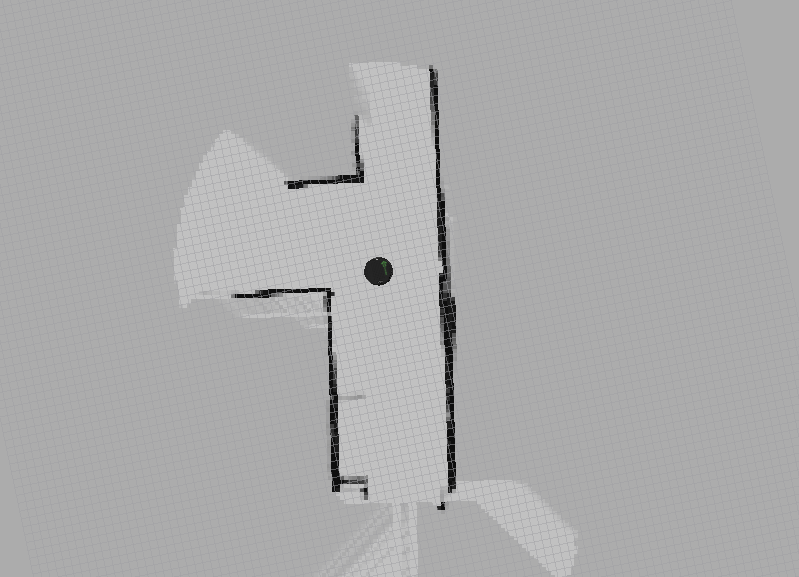
\includegraphics[width=8cm]{img/cap4/costmap-ejemplo}
  \end{center}
  \caption{Ejemplo visual de un costmap.}
  \label{fig:costmap-ejemplo}
\end{figure}\

Para poder representar la ocupación de un objeto en un \textit{costmap} es necesario hacer uso de las transformadas entre frames que nos ofrece ROS.

\subsubsection{tf}
\label{subsubsec:tf}
Cualquier robot está compuesto por multitud de piezas moviles, como puede ser la propia base del robot o la pinza de un brazo robótico. Cada una de estas piezas se pueden representar con un \textit{frame}. Ademas existen tambien otros \textit{frames} que pueden interesarnos, como puede ser el \textit{frame} de world o el \textit{frame} de map.\\
\begin{figure} [hbtp]
  \begin{center}
    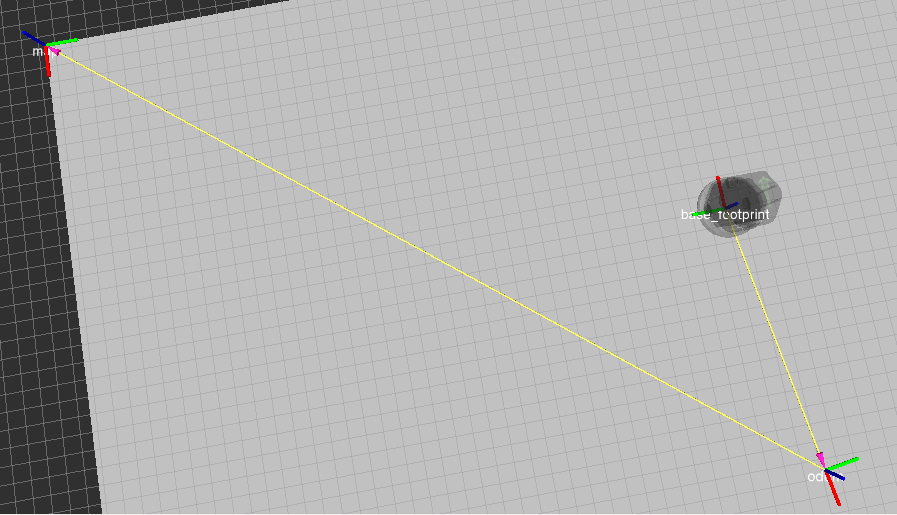
\includegraphics[width=12cm]{img/cap4/frames}
  \end{center}
  \caption{A la izquierda el frame map y a la derecha los frames de odom y base\_footprint}
  \label{fig:frames}
\end{figure}\

Usamos las \textit{tf} para poder representar información relativa a uno de estos frames. Esto puede sernos de utilidad, por ejemplo, si queremos conocer la posición de un objeto que hemos cogido con nuestra pinza respecto a la base de nuestro robot, o cual es la posición relativa de un objeto que estamos percibiendo con el laser respecto a nosotros o respecto al mapa.

Cuando trabajamos con mapas es importante que todo lo que se representa en él sea respecto al frame map. De este modo nuestro mapa puede ser usado por otros nodos, como el nodo de navegación, o en cualquier otro escenario.

\section{Tipos de mapas}

En este apartado se describirá la metodologia seguida para la construcción de cada uno de los tres mapas usados por el algoritmo.

\subsubsection{Mapa estático}
El mapa estático se caracteriza por incluir las partes inmutables del escenario, como son las paredes o las puertas. La mejor manera de construirlo es medir todo el escenario y crear el mapa usando una herramienta de diseño gráfico. En este caso se ha usado \textit{Gimp}.
Este mapa nos servirá como base para crear el mapa de largo plazo.

\begin{figure} [hbtp]
  \begin{center}
    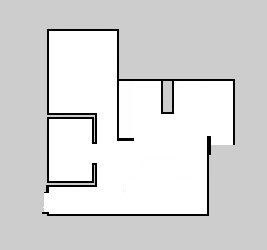
\includegraphics[width=7cm]{img/cap4/mapaestatico}
  \end{center}
  \caption{Mapa estático}
  \label{fig:mapaestatico}
\end{figure}

\subsubsection{Mapa de corto plazo}
El mapa de corto plazo se caracteriza por ser un mapa en el que se representa los objetos que el robot va percibiendo. Este mapa se inicializa con el valor 255, lo que indica una incertidumbre total. En el instante en el que el algoritmo de construcción del mapa comienza a iterar comenzarán a corregirse estos valores iniciales, asignando el valor 0 a las celdas que corresponden con zonas libres e incrementando desde 0 hasta 254 el valor de las celdas que se perciben como ocupadas. \\

{EJEMPLO CODIGO}\\

El algoritmo propuesto destaca por la capacidad de no solo añadir objetos al mapa, si no ademas eliminarlos si los objetos desaparecen del lugar que ocupaban. Para ello se compara cada muestra de datos con el mapa que estamos generando y si en dicha muestra existen celdas libres que en el mapa están ocupadas se decrementa el valor de dicha celda en el mapa. La cuantia del decremento se puede modelar, consiguiendo asi que el robot olvide más lentamente o más rapidamente los objetos que desaparecen del escenario.\\

{EJEMPLO CODIGO}\\
{EJEMPLO GRAFICO}\\




\section{Colección de EKFs}
\label{sec:colecciondeekfs}

Una vez explicada la adaptación del Filtro Extendido de Kalman, ahora hay que integrarlo con el resto del sistema. El EKF, por sí solo, únicamente permite hacer el seguimiento de un objeto. Para poder hacer el seguimiento de varios objetos simultáneamente se utiliza un conjunto de EKFs, cada uno de ellos asociado a uno de los objetos. El conjunto de filtros es dinámico pudiendo ajustarse un número mínimo de observaciones que siempre estarán presentes. En el caso de la pelota es uno, mientras que en el caso de las porterías es dos, poste izquierdo y derecho.\\



Para poder manejar dinámicamente el conjunto de filtros es necesario definir una serie de reglas para añadir un nuevo filtro o para actualizar/eliminar uno de los ya existentes. Hay que tener en cuenta que los filtros creados en el algoritmo puede que no representen un objeto real del entorno, sino que sea un falso positivo. En estos casos, lo ideal es detectarlo cuanto antes y eliminarlo.\\

Realizar el seguimiento de varios objetos es fácil si los objetos no son homogéneos, es decir, si tenemos un método capaz de distinguir cada uno de ellos. Por ejemplo, una pelota azul y una roja. El problema viene cuando realizar la distinción entre varios objetos no es posible. Como por ejemplo pueden ser las lecturas de un radar o los postes de las porterías. El pseudocódigo del algoritmo que se propone en esta investigación se puede ver en Algoritmo \ref{alg:seguimientoobjetos}. Éste puede dividirse en cinco fases:

\begin{packed_item}
\item La instrucción 1 representa la inicialización del algoritmo y se ejecutan una sola vez, al iniciar el algoritmo. Las instrucciones entre las líneas 2 y 22 se ejecutarán en bucle durante todo el período de vida del algoritmo.
\item Entre 2 y 6 se predice el nuevo estado de los objetos que están siguiendo.
\item En las líneas 7 y 14 se incorporan las nuevas observaciones al sistema, ya sea actualizando alguno de los objetos ya existentes o bien, si ninguno satisface las condiciones, creando uno nuevo.
\item Las líneas 15 y 17 añaden ruido a los objetos sospechosos de ser falsos positivos.
\item Por último, entre las líneas 18 y 22 se eliminan los objetos que tengan demasiada incertidumbre.
\end{packed_item}

Además del estado y la incertidumbre de los objetos de seguimiento se guardan algunos datos más que los enriquecen y permite tomar mejores decisiones. Se guarda la marca de tiempo en la que se predijo por última vez el nuevo estado y la marca de tiempo de la última vez que se vio el objeto. También se guarda el \textit{origen} de la observación, que puede ser local o remota. En este proyecto todas las observaciones que se utilizan son locales, pero ésto deja la puerta abierta a futuras mejoras, que se explicarán en el último capítulo. A continuación se detallan cada una de las fases del algoritmo y las operaciones que se realizan en ellas.\\

\subsection{Inicialización de los filtros}
\label{subsec:inicializacion}

La inicialización del algoritmo sólo se produce la primera vez. El algoritmo permite definir un número mínimo de instancias que siempre estarán presentes en la colección. Esta propiedad es útil cuando el sistema donde se integra el algoritmo no permite valores nulos. Un ejemplo sencillo es el caso de la pelota en un partido de la RoboCup. Se sabe que la pelota está siempre presente en el campo. Puede que no se conozca su localización o que esté oculta por el resto de jugadores, pero la pelota está en el terreno de juego. En este caso tiene sentido tener como mínimo una instancia de la pelota en nuestro sistema. En el caso de no haber visto la pelota en mucho tiempo, la instancia tiene almacenada la última posición donde se vio, pero la incertidumbre será tan alta que permite discernir si esa posición es fiable o no.\\

Es necesario inicializar estas instancias con unos valores arbitrarios. La posición inicial de estas instancias no es importante, lo único que hay que tener cuidado es de inicializar la incertidumbre con un valor suficientemente alto para que la instancia no sea fiable y el robot pueda actuar en consecuencia, lo que sería siguiendo la línea del ejemplo anterior, iniciando la búsqueda de la pelota. \\

Otro momento en el que hay que inicializar filtros es cuando tenemos una observación nueva que no corresponde a ninguno de los filtros presentes. Esta operación se describe en \ref{subsubsec:Matching}. En este caso, la inicialización es más sencilla. El filtro se inicializa directamente con los datos de la observación.

\subsection{Predicción de nuevos estados}
\label{subsec:prediccionnuevosestados}

En esta fase, instrucciones entre las líneas 2 y 6, se predice el nuevo estado para cada uno de los objetos sobre los que se está realizando el seguimiento. El estado y la incertidumbre se actualizan mediante la fase de predicción del EKF que ya se ha explicado anteriormente. También se actualiza la marca de tiempo en la que se realiza la predicción.\\

\begin{figure}[h]
  \centering
  \subfloat[El robot está siguiendo dos objetos y se mueve en dirección hacia ellos]{
    \label{fig:prediccion_01}
    %\includegraphics[width=7cm]{img/cap4/prediccion_01}
  }
  \subfloat[Los filtros se encuentran más cerca del robot y ha aumentado su incertidumbre]{
    \label{fig:prediccion_02}
    %\includegraphics[width=7cm]{img/cap4/prediccion_02}
  }
  \caption{Comportamiento de los filtros en la fase de predicción}
  \label{fig:prediccion}
\end{figure}

La figura \ref{fig:prediccion} muestra el comportamiento de los filtros en esta fase. En la imagen de la izquierda el robot está realizando el seguimiento de dos objetos. Cada uno tiene una posición y una incertidumbre. El robot se encuentra moviéndose en dirección a ellos. En la imagen de la derecha se puede ver el resultado de la fase de predicción. Los objetos se encuentran ahora en una posición más cercana al robot, hay que tener en cuenta que las posiciones de los objetos son relativas a éste, y la incertidumbre de los filtros aumenta en consecuencia. \\

\subsection{Incorporación de observaciones}
\label{subsec:incorporacionobservaciones}

En esta fase se realizan varias operaciones para decidir si actualizar un filtro ya existente o, si ninguno satisface las condiciones, crear uno nuevo. Para ello se emparejan las observaciones con los filtros y se calcula el valor de similitud de ellos. Seguidamente se escoge la pareja que más se parezca y, si se cumplen las condiciones necesarias, se actualiza el filtro con la observación. En caso de no cumplirse las condiciones, se crea un filtro nuevo a partir de la observación. Se repite este procedimiento con todas las observaciones. \\

\subsubsection{Emparejamiento}
\label{subsubsec:emparejamiento}

El criterio de emparejamiento utilizado en nuestro algoritmo se basa en la posiciones e incertidumbres tanto de la observación como de cada uno de los filtros. Vincula una observación a uno de los filtros. Para este criterio utilizamos la función de \textit{verosimilitud}, \ref{eq:likelihood}. Esta función permite realizar inferencias acerca del valor de los parámetros de un modelo estadístico a partir de un conjunto de observaciones. En este paso se compara la observación obtenida con todos los filtros y se escoge el que tenga mayor similitud. $s1$ y $P1$ son el estado y la matriz de covarianza de un filtro, respectivamente, y $s2$ y $P2$ representa lo mismo pero de la observación.

\begin{equation}
\label{eq:likelihood}
likelihood = \frac{ e^{ det(-\frac{1}{2} (s1-s2)^T (P1+P2)^I (s1-s2) )} }
                  { \sqrt{ det(2\pi(P1+P2)) } }
\end{equation}

El estado y la matriz de covarianza de cada uno de los filtros no tiene el tamaño original de $4x1$ y $4x4$. Antes de utilizarse en la ecuación se simplifican las matrices eliminando los componentes de velocidad $Vx$ y $Vy$ para que el tamaño de las matrices coincida con los tamaños de las observaciones y pueda aplicarse la ecuación.\\

\begin{figure}[h]
  \centering
  \subfloat[Fusión de una observación con un filtro]{
    \label{fig:emparejamiento_01}
    %\includegraphics[width=7cm]{img/cap4/emparejamiento_01}
  }
  \subfloat[Posible creación de un filtro nuevo]{
    \label{fig:emparejamiento_02}
    %\includegraphics[width=7cm]{img/cap4/emparejamiento_02}
  }
  \caption{Distintas situaciones del emparejamiento entre una observación y un filtro}
  \label{fig:emparejamientos}
\end{figure}

En la figura \ref{fig:emparejamientos} se puede ver un ejemplo gráfico más fácil de entender. En las imágenes aparecen una colección de tres filtros y dos situaciones distintas al incorporar dos observaciones distintas. En la figura \ref{fig:emparejamiento_01} se ve claramente que la observación se emparejaría con el filtro 1. En la figura \ref{fig:emparejamiento_02} la situación no está tan clara. La observación se encuentra prácticamente a la misma distancia de todos ellos. La observación se emparejaría con el filtro 3 por ser el que más incertidumbre tiene.

\subsubsection{Matching}
\label{subsubsec:Matching}

Una vez que se ha escogido uno de los filtros existentes hay que decidir si actualizarlo con la nueva observación o crear una filtro nuevo. El método que utilizamos es bastante simple e intuitivo. Se comprueba si las elipses generadas a partir de la media y covarianza de la observación y del filtro intersectan, en cuyo caso se considera que ambas se corresponden con el mismo objeto y se actualiza el filtro con la observación. En caso contrario, se crearía un nuevo filtro. \\

Al calcular la intersección de las elipses, el tamaño de éstas se multiplica por 4 siguiendo la desigualdad de Chebyshev. Este factor es un resultado que ofrece una cota inferior a la probabilidad de que el valor de una variable aleatoria con varianza finita esté a una cierta distancia de su esperanza matemática. En la siguiente ecuación, se puede ver el valor de la desigualdad de Chebyshev para un valor $k$ veces la desviación típica partiendo de la media. En nuestro caso, hemos escogido el valor 4 y devuelve un resultado muy próximo a $94\%$. \\

\begin{tabular}{cc}
  \textbf{Población mínima} & \textbf{\# de desviaciones típicas desde la media} \\
  50\% & $\sqrt{2}$ \\
  75\% & 2 \\ 
  89\% & 3 \\
  94\% & 4 \\
  96\% & 5 \\
  97\% & 6 \\
  $1-\frac{1}{k^2}$ & k \\
  l & $\frac{1}{\sqrt{1-l}}$
\end{tabular}
\\

Esta tabla se puede leer: para cualquier distribución con una desviación estándar definida, la cantidad de datos que se encuentran a una distancia $k$ veces la desviación típica de la media es, al menos, como se indica en la tabla. Es decir, a una distancia 4 veces la desviación típica partiendo de la media se encuentran el 94\% de los datos. \\

La intersección de dos elipses no es un cálculo sencillo. Hay que tener en cuenta distintos casos: cuando la distancia entre las elipses es demasiado grande para intersectar, cuando el centro de una ellas está contenida dentro de la otra que intersecta siempre, o cuando simplemente intersectan en uno, dos, tres o cuatro puntos. Las elipses están definidas por 5 parámetros: $x$ e $y$, que son las coordenadas del centro; $a$  $b$, que son los semi-ejes mayor y menor respectivamente, y $\lambda$ que es la rotación. \\

\begin{enumerate}

\item Primero se comprueba que las elipses estén a una distancia mínima en la puedan intersectarse o una esté contenida dentro de la otra. En caso de no cumplirse este requisito, se puede afirmar que las elipses no intersectan. Por lo que si la distancia entre los centros es mayor que la suma de los dos semi-ejes de mayor tamaño, las elipses no intersectan.
\begin{equation}
  \sqrt{ (x_1 - x_2)^2 + (y_1 - y_2)^2 } > a_1 + a_2 \rightarrow \text{no intersectan}
\end{equation}

\item Si el centro de una de las elipses está contenido dentro de la otra, entonces se puede afirmar que las elipses intersectan o una está contenida totalmente dentro de la otra, situación igualmente válida. $p$ y $q$ son las coordenadas del centro de la otra elipse.
\begin{equation}
  \frac{ ((p \cos \lambda + q \sin \lambda ) - x)^2 }{ a^2 } + 
  \frac{ ((p \sin \lambda - q \cos \lambda ) - y)^2 }{ b^2 } \leq 1
\end{equation}

\item Por último, si en caso de no poder afirmar nada aún hay que resolver los puntos de intersección de las elipses. A partir de las ecuaciones de la elipse en su forma
\begin{equation}
  \begin{split}
  ax^2  + bxy  + cy^2  + dx  + ey  + f = 0 \\
  a'x^2 + b'xy + c'y^2 + d'x + e'y + f' = 0    
  \end{split}
\end{equation}

se obtiene una ecuación de cuarto grado que puede resolverse en forma cerrada. Esto quiere decir que se puede resolver en términos de funciones y operaciones matemáticas elegidas de un conjunto limitado. Una ecuación de cuarto grado tiene la siguiente forma
\begin{equation}
  ax^4 + bx^3 + cx^2 + dx + e = 0
\end{equation}

Se pueden hacer una serie de comprobaciones rápidas en la ecuación para averiguar tiene soluciones no triviales.
\begin{itemize}
\item Si $e = 0$ una de las raíces es $0$, por lo tanto intersectan por lo menos en un punto.
\item Si $a=0$, $b \neq 0$, se trata de una ecuación cúbica que siempre tiene raíces.
\item Si $a=0$, $b=0$, $c \neq 0$, ecuación cuadrática. Sencillo de resolver mediante la fórmula cuadrática $x=\frac{-b \pm \sqrt{b^2 - 4ac}}{2a}$
\item Si $a=0$, $b=0$, $c=0$ y $d \neq 0$, todas las rectas con pendiente distinta de 0 tienen una raíz
\end{itemize}

En cualquier otro caso hay que resolver la ecuación de cuarto grado, operación más costosa computacionalmente.

\end{enumerate}

\subsection{Descarte de filtros}
\label{subsec:descartefiltros}

Para obtener un rendimiento mayor es necesario tener el menor número de filtros posibles ejecutándose al mismo tiempo. En caso de no borrarse ningún filtro, al ser una colección dinámica, el tamaño podría crecer desmesuradamente en un corto espacio de tiempo perjudicando enormemente el rendimiento del algoritmo. Normalmente se quiere eliminar un filtro cuando se trata de un falso positivo o cuando un objeto sobre el que se estaba realizando el seguimiento desaparece del entorno.\\

La colección de filtros tiene un número mínimo de objetos sobre los que hace el seguimiento. Este límite es útil para situaciones en las que se puede afirmar que siempre estará presente en el entorno ese mínimo número de objetos, como, por ejemplo, cuando se realiza el seguimiento de una pelota en un partido de la RoboCup. Siempre hay una pelota, aunque el robot no la haya localizado o la haya perdido de vista. En el caso de haber localizado en algún momento la pelota, pero haberla perdido de vista hace un tiempo, el filtro almacena la última posición conocida de la pelota. Al haberse perdido de vista hace tiempo la pelota tendrá una incertidumbre alta. Esta información es muy útil para comportamientos de más alto nivel ya que pueden basar sus decisiones, además de en la posición de la pelota, en su incertidumbre.\\

El método utilizado es bastante simple. Si hay un número mayor de filtros que el número mínimo especificado, se compara el área de la elipse con un umbral determinado y, en caso de superarse, el filtro se elimina. Este umbral se elige de forma arbitraria. El método usado para que sea sencillo elegir el umbral es crearlo a partir del área de una circunferencia. Dependiendo del modelo del objeto que se utilice se puede tener un umbral más alto o más bajo, pudiendo adaptarse el algoritmo a mayor cantidad de problemas.

\begin{equation}
  \underbrace{2ab}_{\text{Área elipse}} > \underbrace{\pi r^2}_{\text{Área circunferencia}} \rightarrow \text{eliminar filtro}
\end{equation}

\section{Adición de incertidumbre}
\label{sec:adicionincertidumbre}

El algoritmo del Filtro de Kalman está pensado para tener una fuente de datos continua. En cada iteración se actualiza la información del filtro con las nuevas observaciones. El problema es que normalmente un robot tiene una visión parcial del problema y puede no percibir todos los objetos todo el tiempo. El algoritmo básico de Kalman no contempla esta situación. La única manera de aumentar la incertidumbre es mediante el movimiento del robot o mediante otras observaciones. Pero, ¿qué pasa cuando un robot está parado y no detecta un objeto? La forma más sencilla de entenderlo es mediante un ejemplo. \\

Durante un partido de fútbol suponemos que el portero tiene localizada la pelota con muy poca incertidumbre. En ese momento se empiezan a juntar jugadores alrededor de ella, provocando que el portero la pierda de vista. Si el portero está estático, al no tener ninguna observación de la pelota, el filtro mantiene el mismo estado y la misma incertidumbre a lo largo del tiempo. En ese período de tiempo lo más probable es que la pelota se haya movido del sitio en el que estaba, pero el portero sigue con una incertidumbre muy baja lo que le lleva a tomar decisiones como si la pelota siguiese en ese sitio. Decisiones probablemente desacertadas. \\

Otro comportamiento que se ha observado que no favorece el seguimiento de objetos con movimiento se produce cuando se observa un objeto durante un período de tiempo seguido en el mismo sitio. El filtro tiende a disminuir demasiado la incertidumbre provocando que no sea reactivo a nuevos movimientos del objeto. En nuestra implementación en concreto, se generaba un nuevo filtro para el mismo objeto. \\

En el primero de los casos, el comportamiento buscado es aumentar la incertidumbre del objeto cuando éste no se visualice. De esta manera, el portero, podría reaccionar frente a la situación de perder de vista la pelota entre los jugadores. En todo momento sigue recordando la última posición en la que ésta se encontraba, pero es capaz de reaccionar mucho antes a las nuevas situaciones que se presenten. Por otro lado, en el segundo caso, también se busca introducir un poco de ruido en los filtros para mantenerlos más reactivos, sobre todo aquellos que tienen más movimiento. \\

Se han definido tres niveles de adición de incertidumbre distintos dependiendo de la situación:
\begin{enumerate}

\item El filtro se ha actualizado con una observación. En este caso se añade un mínimo de ruido para mantener el filtro reactivo. La cantidad de incertidumbre depende de los valores con los que se ha modelado el objeto.

\item El filtro no se ha actualizado porque no se encuentra en el \textit{frustum} de la cámara. De un objeto en esta situación no se puede afirmar nada, si sigue en el mismo lugar o se ha desplazado, por lo que se añade una cantidad \textit{estándar} de ruido.

\item Si un filtro no se actualiza y debería estar en la imagen. Esta situación la tomamos como un falso positivo. Puede que en realidad el filtro no sea un falso positivo y sea una oclusión o que el detector no lo localice en la imagen, pero es muy difícil discernir entre estas posibilidades.

\end{enumerate}

En esta fase se decide en cuál de las tres situaciones se encuentra cada uno de los filtros y se suma el ruido correspondiente a la matriz de covarianza del filtro:
\begin{equation}
  S' = S + noise^{\# \text{situación}} I
\end{equation}

\section{Objetos complejos}
\label{sec:objetoscomplejos}

En ocasiones se quieren seguir objetos que están compuestos de formas más simples y más sencillas de reconocer. Esto se hace porque el objeto es demasiado grande y no puede ser detectado con una sola imagen, o bien porque es demasiado complejo para resolver el problema de una vez y se divide en problemas más sencillos. \\

En el caso de las porterías en el fútbol se dan los dos casos expuestos. Detectar una portería al completo es una tarea bastante difícil, ya que habría que detectar los dos postes al mismo tiempo para poder detectar que ese objeto es una portería. Pero los postes están separados por una distancia considerable y dependiendo de la distancia a la que se encuentre el robot de éstos, puede ser imposible ver los dos postes al mismo tiempo. Por esto se ha simplificado el problema inicial en hacer el seguimiento de los postes y, a partir de estos, averiguar los dos postes con más probabilidades de ser una portería.

\begin{figure} [h]
  \centering
  %\includegraphics[width=15cm]{img/cap4/prod_vectorial}
  \caption{Distinguir poste izquierdo de poste derecho}
  \label{fig:prod_vectorial}
\end{figure}

Para ello se crea una colección de filtros con un mínimo de dos instancias de los postes de la portería. Simplemente se siguen los postes sin tener en cuenta si son de una portería o no. \textit{A posteriori} se realiza una serie de cálculos para, de entre todos los postes de la colección, decidir cuáles son más probables de ser una portería. Se realiza la siguiente operación a cada uno de las combinaciones de postes que haya en la colección. $s$ es la posición del poste y $P$ su covarianza.
\begin{equation}
  \begin{split}
    s' = f(s_1 - s_2) \\
    P' = A (P_1 + P_2) A^T 
  \end{split}
\end{equation}

donde $f()$ es la función para pasar del espacio euclídeo $\mathbb{R}^2 \rightarrow \mathbb{R}^1$ y $A$ es la matriz jacobiana de la función
\begin{equation}
  \begin{split}
    f(s) = \sqrt{s_x^2 + s_y^2} \\
    A = \begin{pmatrix} \frac{s_x}{\sqrt{s_x^2 + s_y^2}} & \frac{s_y}{\sqrt{s_x^2 + s_y^2}} \end{pmatrix}    
  \end{split}
\end{equation}

Una vez hecho esto, para cada par de postes de la colección se tiene la distancia entre ellos y la covarianza de ésta. Para decidir qué par de postes es el que más se parece a una portería, se utiliza el mismo método que cuando se emparejan las observaciones con los filtros, se calcula de la distancia de \textit{Mahalanobis}. 

%Poner flecha de vector a x e y.
\begin{equation}
  d(x,y) = \sqrt{(x-y)^T S^{-1} (x-y)}
\end{equation}

Esta distancia es un método estadístico descriptivo que aporta una medición relativa de varios puntos a uno común. El valor calculado no tiene unidades de medida, lo que lo convierte en un método muy útil para comparar distancias teniendo en cuenta la incertidumbre. En nuestro caso se calcula el error de distancia entre los dos postes, $1500 - dist(post1,post2)$. \\

Una vez escogidos los postes que van a representar la portería, hay que diferenciar el izquierdo del derecho. Se calcula mediante el producto vectorial entre los dos postes. Si el producto entre el poste 1 y el poste 2 es positivo, entonces el poste 1 es el derecho y el poste 2 es el izquierdo. Si el producto es negativo, es a la inversa. La figura \ref{fig:prod_vectorial} muestra el cálculo.
